% Generated by paper/figures/make-fig-phase1.py from evidence/mean-square-boundary/raw-phase1.json; do not edit.
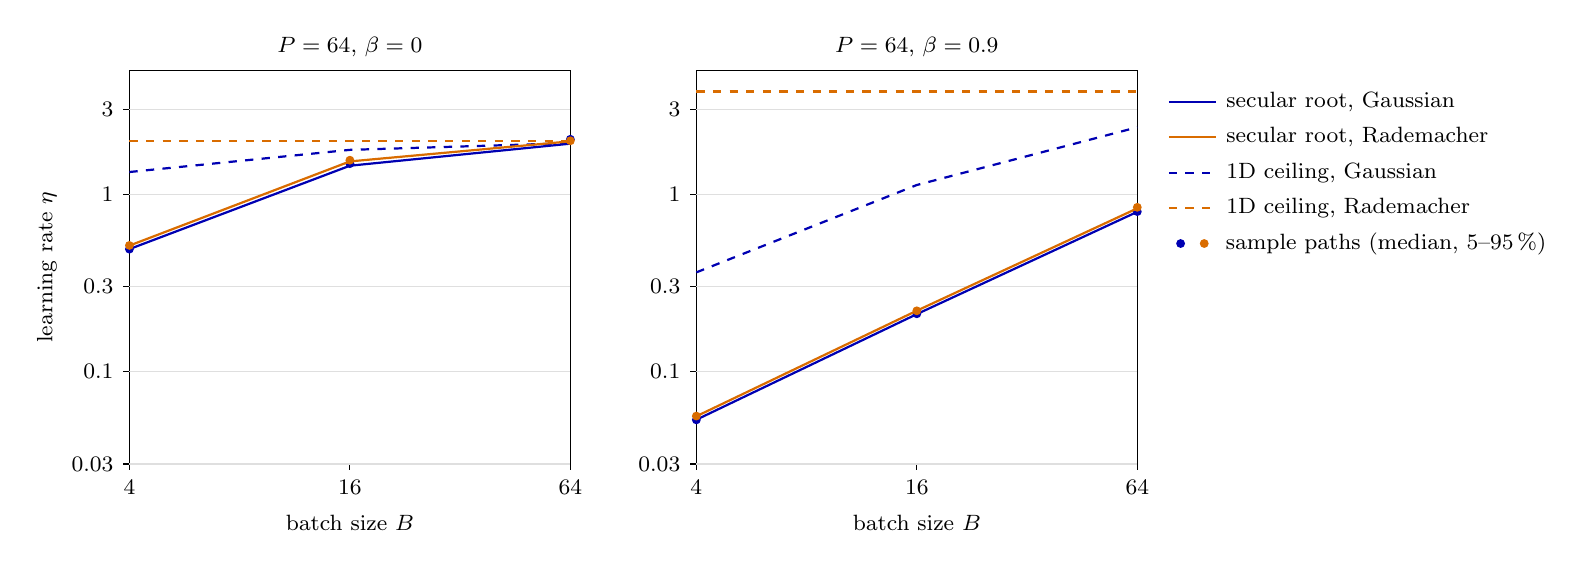
\begin{tikzpicture}[font=\footnotesize]
\tikzset{gauss/.style={blue!70!black}, radem/.style={orange!85!black}}
\draw (0.0,0) rectangle (5.6,5.0);
\draw (0.0000,0) -- (0.0000,-0.08) node[below] {4};
\draw (2.8000,0) -- (2.8000,-0.08) node[below] {16};
\draw (5.6000,0) -- (5.6000,-0.08) node[below] {64};
\draw[gray!25] (0.0,0.0000) -- (5.6,0.0000);
\draw (0.0,0.0000) -- (-0.08,0.0000) node[left] {0.03};
\draw[gray!25] (0.0,1.1767) -- (5.6,1.1767);
\draw (0.0,1.1767) -- (-0.08,1.1767) node[left] {0.1};
\draw[gray!25] (0.0,2.2504) -- (5.6,2.2504);
\draw (0.0,2.2504) -- (-0.08,2.2504) node[left] {0.3};
\draw[gray!25] (0.0,3.4271) -- (5.6,3.4271);
\draw (0.0,3.4271) -- (-0.08,3.4271) node[left] {1};
\draw[gray!25] (0.0,4.5008) -- (5.6,4.5008);
\draw (0.0,4.5008) -- (-0.08,4.5008) node[left] {3};
\node at (2.8,-0.75) {batch size $B$};
\node[anchor=south] at (2.8,5.05) {$P=64$, $\beta=0$};
\node[rotate=90] at (-1.05,2.5) {learning rate $\eta$};
\draw[gauss, dashed, thick] (0.0000,3.7082) -- (2.8000,3.9894) -- (5.6000,4.0744);
\draw[gauss, thick] (0.0000,2.7292) -- (2.8000,3.7880) -- (5.6000,4.0681);
\draw[gauss] (0.0000,2.7249) -- (0.0000,2.7412);
\fill[gauss] (0.0000,2.7287) circle (1.6pt);
\draw[gauss] (2.8000,3.7900) -- (2.8000,3.8213);
\fill[gauss] (2.8000,3.8143) circle (1.6pt);
\draw[gauss] (5.6000,4.0972) -- (5.6000,4.1238);
\fill[gauss] (5.6000,4.1238) circle (1.6pt);
\draw[radem, dashed, thick] (0.0000,4.1045) -- (2.8000,4.1045) -- (5.6000,4.1045);
\draw[radem, thick] (0.0000,2.7735) -- (2.8000,3.8426) -- (5.6000,4.0977);
\draw[radem] (0.0000,2.7730) -- (0.0000,2.7807);
\fill[radem] (0.0000,2.7756) circle (1.6pt);
\draw[radem] (2.8000,3.8425) -- (2.8000,3.8645);
\fill[radem] (2.8000,3.8581) circle (1.6pt);
\draw[radem] (5.6000,4.0979) -- (5.6000,4.1116);
\fill[radem] (5.6000,4.1047) circle (1.6pt);
\draw (7.199999999999999,0) rectangle (12.799999999999999,5.0);
\draw (7.2000,0) -- (7.2000,-0.08) node[below] {4};
\draw (10.0000,0) -- (10.0000,-0.08) node[below] {16};
\draw (12.8000,0) -- (12.8000,-0.08) node[below] {64};
\draw[gray!25] (7.199999999999999,0.0000) -- (12.799999999999999,0.0000);
\draw (7.199999999999999,0.0000) -- (7.119999999999999,0.0000) node[left] {0.03};
\draw[gray!25] (7.199999999999999,1.1767) -- (12.799999999999999,1.1767);
\draw (7.199999999999999,1.1767) -- (7.119999999999999,1.1767) node[left] {0.1};
\draw[gray!25] (7.199999999999999,2.2504) -- (12.799999999999999,2.2504);
\draw (7.199999999999999,2.2504) -- (7.119999999999999,2.2504) node[left] {0.3};
\draw[gray!25] (7.199999999999999,3.4271) -- (12.799999999999999,3.4271);
\draw (7.199999999999999,3.4271) -- (7.119999999999999,3.4271) node[left] {1};
\draw[gray!25] (7.199999999999999,4.5008) -- (12.799999999999999,4.5008);
\draw (7.199999999999999,4.5008) -- (7.119999999999999,4.5008) node[left] {3};
\node at (10.0,-0.75) {batch size $B$};
\node[anchor=south] at (10.0,5.05) {$P=64$, $\beta=0.9$};
\draw[gauss, dashed, thick] (7.2000,2.4337) -- (10.0000,3.5430) -- (12.8000,4.2763);
\draw[gauss, thick] (7.2000,0.5622) -- (10.0000,1.9033) -- (12.8000,3.2026);
\draw[gauss] (7.2000,0.5542) -- (7.2000,0.5696);
\fill[gauss] (7.2000,0.5603) circle (1.6pt);
\draw[gauss] (10.0000,1.8984) -- (10.0000,1.9325);
\fill[gauss] (10.0000,1.9076) circle (1.6pt);
\draw[gauss] (12.8000,3.1915) -- (12.8000,3.2194);
\fill[gauss] (12.8000,3.2054) circle (1.6pt);
\draw[radem, dashed, thick] (7.2000,4.7318) -- (10.0000,4.7318) -- (12.8000,4.7318);
\draw[radem, thick] (7.2000,0.6058) -- (10.0000,1.9469) -- (12.8000,3.2467);
\draw[radem] (7.2000,0.5953) -- (7.2000,0.6166);
\fill[radem] (7.2000,0.6086) circle (1.6pt);
\draw[radem] (10.0000,1.9375) -- (10.0000,1.9615);
\fill[radem] (10.0000,1.9455) circle (1.6pt);
\draw[radem] (12.8000,3.2335) -- (12.8000,3.2685);
\fill[radem] (12.8000,3.2599) circle (1.6pt);
\draw[gauss, thick] (13.2,4.6) -- (13.799999999999999,4.6) node[right, black] {secular root, Gaussian};
\draw[radem, thick] (13.2,4.1499999999999995) -- (13.799999999999999,4.1499999999999995) node[right, black] {secular root, Rademacher};
\draw[gauss, dashed, thick] (13.2,3.6999999999999997) -- (13.799999999999999,3.6999999999999997) node[right, black] {1D ceiling, Gaussian};
\draw[radem, dashed, thick] (13.2,3.2499999999999996) -- (13.799999999999999,3.2499999999999996) node[right, black] {1D ceiling, Rademacher};
\fill[gauss] (13.35,2.8) circle (1.6pt); \fill[radem] (13.649999999999999,2.8) circle (1.6pt);
\node[right] at (13.799999999999999,2.8) {sample paths (median, 5--95\,\%)};
\end{tikzpicture}
